\begin{figure}[htbp]
    \centering
    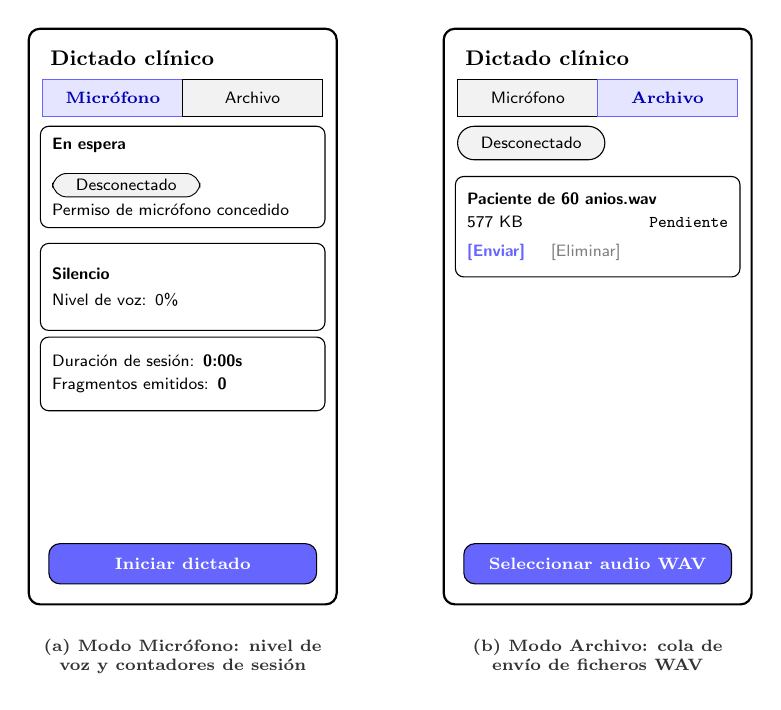
\begin{tikzpicture}[
        scale=0.85, transform shape,
        font=\sffamily\scriptsize,
        title/.style={font=\bfseries\small},
        tab/.style={draw, fill=black!5, minimum width=2.1cm, minimum height=0.55cm, align=center},
        tabActive/.style={tab, fill=blue!10, draw=blue!60, text=blue!70!black, font=\bfseries\scriptsize},
        pill/.style={draw, rounded corners=6pt, fill=black!5, minimum width=2.2cm, minimum height=0.5cm, align=center},
        card/.style={draw, rounded corners=3pt, fill=white, text width=3.9cm, align=left, inner sep=5pt, anchor=north},
        btn/.style={draw, fill=blue!60, text=white, rounded corners=4pt, minimum width=4cm, minimum height=0.6cm, font=\bfseries\scriptsize},
        lbl/.style={align=center, font=\scriptsize\bfseries\color{black!80}}
    ]

        % ========================================================
        % MARCOS DE PANTALLA
        % ========================================================
        \draw[thick, rounded corners=4pt, fill=white] (-2.3,-4.3) rectangle (2.3,4.3);
        \draw[thick, rounded corners=4pt, fill=white] (3.9,-4.3) rectangle (8.5,4.3);

        % ========================================================
        % PANTALLA A: MODO MICRÓFONO
        % ========================================================
        \node[title, anchor=north west] at (-2.1, 4.1) {Dictado clínico};

        \node[tabActive, anchor=north west] at (-2.1, 3.55) {Micrófono};
        \node[tab, anchor=north east] at (2.1, 3.55) {Archivo};

        \node[card, minimum height=1.5cm] at (0, 2.85) {
            \textbf{En espera}\\[2pt]
            \tikz[baseline]{\node[pill, minimum height=0.35cm, font=\scriptsize, inner sep=0pt]{Desconectado};}\\[2pt]
            Permiso de micrófono concedido
        };

        \node[card, minimum height=1.3cm] at (0, 1.1) {
            \textbf{Silencio}\\[3pt]
            Nivel de voz: 0\%
        };

        \node[card, minimum height=1.1cm] at (0, -0.3) {
            Duración de sesión: \textbf{0:00s}\\[2pt]
            Fragmentos emitidos: \textbf{0}
        };

        \node[btn, anchor=south] at (0, -4.0) {Iniciar dictado};

        \node[lbl, anchor=north] at (0, -4.7) {(a) Modo Micrófono: nivel de\\ voz y contadores de sesión};

        % ========================================================
        % PANTALLA B: MODO ARCHIVO
        % ========================================================
        \node[title, anchor=north west] at (4.1, 4.1) {Dictado clínico};

        \node[tab, anchor=north west] at (4.1, 3.55) {Micrófono};
        \node[tabActive, anchor=north east] at (8.3, 3.55) {Archivo};

        \node[pill, anchor=north west] at (4.1, 2.85) {Desconectado};

        \node[card, minimum height=1.5cm] at (6.2, 2.1) {
            \textbf{Paciente de 60 anios.wav}\\[2pt]
            577 KB \hfill \texttt{Pendiente}\\[4pt]
            \textcolor{blue!60}{\textbf{[Enviar]}} \hspace{6pt} \textcolor{black!50}{[Eliminar]}
        };

        \node[btn, anchor=south] at (6.2, -4.0) {Seleccionar audio WAV};

        \node[lbl, anchor=north] at (6.2, -4.7) {(b) Modo Archivo: cola de\\ envío de ficheros WAV};

    \end{tikzpicture}
    \caption{Wireframe de las dos pantallas de captura de la aplicación móvil: selección de fichero pregrabado (a) y captura en tiempo real con monitorización de VAD (b).}
    \label{fig:wireframes_app}
\end{figure}
